\documentclass[twoside]{book}

% Packages required by doxygen
\usepackage{fixltx2e}
\usepackage{calc}
\usepackage{doxygen}
\usepackage[export]{adjustbox} % also loads graphicx
\usepackage{graphicx}
\usepackage[utf8]{inputenc}
\usepackage{makeidx}
\usepackage{multicol}
\usepackage{multirow}
\PassOptionsToPackage{warn}{textcomp}
\usepackage{textcomp}
\usepackage[nointegrals]{wasysym}
\usepackage[table]{xcolor}

% Font selection
\usepackage[T1]{fontenc}
\usepackage[scaled=.90]{helvet}
\usepackage{courier}
\usepackage{amssymb}
\usepackage{sectsty}
\renewcommand{\familydefault}{\sfdefault}
\allsectionsfont{%
  \fontseries{bc}\selectfont%
  \color{darkgray}%
}
\renewcommand{\DoxyLabelFont}{%
  \fontseries{bc}\selectfont%
  \color{darkgray}%
}
\newcommand{\+}{\discretionary{\mbox{\scriptsize$\hookleftarrow$}}{}{}}

% Page & text layout
\usepackage{geometry}
\geometry{%
  a4paper,%
  top=2.5cm,%
  bottom=2.5cm,%
  left=2.5cm,%
  right=2.5cm%
}
\tolerance=750
\hfuzz=15pt
\hbadness=750
\setlength{\emergencystretch}{15pt}
\setlength{\parindent}{0cm}
\setlength{\parskip}{3ex plus 2ex minus 2ex}
\makeatletter
\renewcommand{\paragraph}{%
  \@startsection{paragraph}{4}{0ex}{-1.0ex}{1.0ex}{%
    \normalfont\normalsize\bfseries\SS@parafont%
  }%
}
\renewcommand{\subparagraph}{%
  \@startsection{subparagraph}{5}{0ex}{-1.0ex}{1.0ex}{%
    \normalfont\normalsize\bfseries\SS@subparafont%
  }%
}
\makeatother

% Headers & footers
\usepackage{fancyhdr}
\pagestyle{fancyplain}
\fancyhead[LE]{\fancyplain{}{\bfseries\thepage}}
\fancyhead[CE]{\fancyplain{}{}}
\fancyhead[RE]{\fancyplain{}{\bfseries\leftmark}}
\fancyhead[LO]{\fancyplain{}{\bfseries\rightmark}}
\fancyhead[CO]{\fancyplain{}{}}
\fancyhead[RO]{\fancyplain{}{\bfseries\thepage}}
\fancyfoot[LE]{\fancyplain{}{}}
\fancyfoot[CE]{\fancyplain{}{}}
\fancyfoot[RE]{\fancyplain{}{\bfseries\scriptsize Generated by Doxygen }}
\fancyfoot[LO]{\fancyplain{}{\bfseries\scriptsize Generated by Doxygen }}
\fancyfoot[CO]{\fancyplain{}{}}
\fancyfoot[RO]{\fancyplain{}{}}
\renewcommand{\footrulewidth}{0.4pt}
\renewcommand{\chaptermark}[1]{%
  \markboth{#1}{}%
}
\renewcommand{\sectionmark}[1]{%
  \markright{\thesection\ #1}%
}

% Indices & bibliography
\usepackage{natbib}
\usepackage[titles]{tocloft}
\setcounter{tocdepth}{3}
\setcounter{secnumdepth}{5}
\makeindex

% Hyperlinks (required, but should be loaded last)
\usepackage{ifpdf}
\ifpdf
  \usepackage[pdftex,pagebackref=true]{hyperref}
\else
  \usepackage[ps2pdf,pagebackref=true]{hyperref}
\fi
\hypersetup{%
  colorlinks=true,%
  linkcolor=blue,%
  citecolor=blue,%
  unicode%
}

% Custom commands
\newcommand{\clearemptydoublepage}{%
  \newpage{\pagestyle{empty}\cleardoublepage}%
}

\usepackage{caption}
\captionsetup{labelsep=space,justification=centering,font={bf},singlelinecheck=off,skip=4pt,position=top}

%===== C O N T E N T S =====

\begin{document}

% Titlepage & ToC
\hypersetup{pageanchor=false,
             bookmarksnumbered=true,
             pdfencoding=unicode
            }
\pagenumbering{alph}
\begin{titlepage}
\vspace*{7cm}
\begin{center}%
{\Large Template }\\
\vspace*{1cm}
{\large Generated by Doxygen 1.8.13}\\
\end{center}
\end{titlepage}
\clearemptydoublepage
\pagenumbering{roman}
\tableofcontents
\clearemptydoublepage
\pagenumbering{arabic}
\hypersetup{pageanchor=true}

%--- Begin generated contents ---
\chapter{Class Index}
\section{Class List}
Here are the classes, structs, unions and interfaces with brief descriptions\+:\begin{DoxyCompactList}
\item\contentsline{section}{\hyperlink{struct_s_t_r_u___c_s_v___c_o_u_n_t}{S\+T\+R\+U\+\_\+\+C\+S\+V\+\_\+\+C\+O\+U\+NT} }{\pageref{struct_s_t_r_u___c_s_v___c_o_u_n_t}}{}
\item\contentsline{section}{\hyperlink{struct_s_t_r_u___d_e_m_o}{S\+T\+R\+U\+\_\+\+D\+E\+MO} }{\pageref{struct_s_t_r_u___d_e_m_o}}{}
\end{DoxyCompactList}

\chapter{File Index}
\section{File List}
Here is a list of all files with brief descriptions\+:\begin{DoxyCompactList}
\item\contentsline{section}{\hyperlink{sd__app_8c}{sd\+\_\+app.\+c} \\*Sd\+\_\+card functions for application }{\pageref{sd__app_8c}}{}
\item\contentsline{section}{\hyperlink{sd__app_8h}{sd\+\_\+app.\+h} }{\pageref{sd__app_8h}}{}
\item\contentsline{section}{\hyperlink{sd__manage__lib_8c}{sd\+\_\+manage\+\_\+lib.\+c} \\*Contain functions to manage read and write sd card action }{\pageref{sd__manage__lib_8c}}{}
\item\contentsline{section}{\hyperlink{sd__manage__lib_8h}{sd\+\_\+manage\+\_\+lib.\+h} }{\pageref{sd__manage__lib_8h}}{}
\end{DoxyCompactList}

\chapter{Class Documentation}
\hypertarget{struct_s_t_r_u___d_e_m_o}{}\section{S\+T\+R\+U\+\_\+\+D\+E\+MO Struct Reference}
\label{struct_s_t_r_u___d_e_m_o}\index{S\+T\+R\+U\+\_\+\+D\+E\+MO@{S\+T\+R\+U\+\_\+\+D\+E\+MO}}


{\ttfamily \#include $<$header\+\_\+template.\+h$>$}

\subsection*{Public Attributes}
\begin{DoxyCompactItemize}
\item 
uint8\+\_\+t \hyperlink{struct_s_t_r_u___d_e_m_o_a79ae9788d6fe743339242fc3369a482e}{u8\+\_\+demo\+\_\+value}
\end{DoxyCompactItemize}


\subsection{Detailed Description}
A description of the struct. 

\subsection{Member Data Documentation}
\mbox{\Hypertarget{struct_s_t_r_u___d_e_m_o_a79ae9788d6fe743339242fc3369a482e}\label{struct_s_t_r_u___d_e_m_o_a79ae9788d6fe743339242fc3369a482e}} 
\index{S\+T\+R\+U\+\_\+\+D\+E\+MO@{S\+T\+R\+U\+\_\+\+D\+E\+MO}!u8\+\_\+demo\+\_\+value@{u8\+\_\+demo\+\_\+value}}
\index{u8\+\_\+demo\+\_\+value@{u8\+\_\+demo\+\_\+value}!S\+T\+R\+U\+\_\+\+D\+E\+MO@{S\+T\+R\+U\+\_\+\+D\+E\+MO}}
\subsubsection{\texorpdfstring{u8\+\_\+demo\+\_\+value}{u8\_demo\_value}}
{\footnotesize\ttfamily uint8\+\_\+t S\+T\+R\+U\+\_\+\+D\+E\+M\+O\+::u8\+\_\+demo\+\_\+value}

Some documentation for u8\+\_\+demo\+\_\+value 

The documentation for this struct was generated from the following file\+:\begin{DoxyCompactItemize}
\item 
\hyperlink{header__template_8h}{header\+\_\+template.\+h}\end{DoxyCompactItemize}

\chapter{File Documentation}
\hypertarget{c__template_8c}{}\section{c\+\_\+template.\+c File Reference}
\label{c__template_8c}\index{c\+\_\+template.\+c@{c\+\_\+template.\+c}}
{\ttfamily \#include $<$stdint.\+h$>$}\newline
Include dependency graph for c\+\_\+template.\+c\+:\nopagebreak
\begin{figure}[H]
\begin{center}
\leavevmode
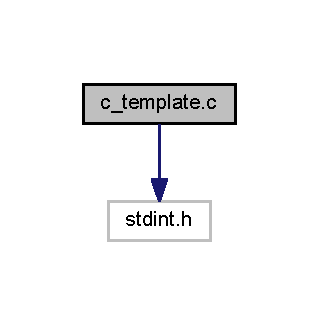
\includegraphics[width=153pt]{c__template_8c__incl}
\end{center}
\end{figure}
\subsection*{Functions}
\begin{DoxyCompactItemize}
\item 
void \hyperlink{c__template_8c_acd5f726f1523ec7ab28b27ab1b42f317}{v\+\_\+function\+\_\+demo} (uint8\+\_\+t u8\+\_\+var1, uint32\+\_\+t u32\+\_\+var2)
\begin{DoxyCompactList}\small\item\em Description of function. \end{DoxyCompactList}\end{DoxyCompactItemize}


\subsection{Function Documentation}
\mbox{\Hypertarget{c__template_8c_acd5f726f1523ec7ab28b27ab1b42f317}\label{c__template_8c_acd5f726f1523ec7ab28b27ab1b42f317}} 
\index{c\+\_\+template.\+c@{c\+\_\+template.\+c}!v\+\_\+function\+\_\+demo@{v\+\_\+function\+\_\+demo}}
\index{v\+\_\+function\+\_\+demo@{v\+\_\+function\+\_\+demo}!c\+\_\+template.\+c@{c\+\_\+template.\+c}}
\subsubsection{\texorpdfstring{v\+\_\+function\+\_\+demo()}{v\_function\_demo()}}
{\footnotesize\ttfamily v\+\_\+function\+\_\+demo (\begin{DoxyParamCaption}\item[{uint8\+\_\+t}]{u8\+\_\+var1,  }\item[{uint32\+\_\+t}]{u32\+\_\+var2 }\end{DoxyParamCaption})}



Description of function. 

Global functions


\begin{DoxyParams}[1]{Parameters}
\mbox{\tt in}  & {\em u8\+\_\+var1} & description for u8\+\_\+var1 \\
\hline
\mbox{\tt in}  & {\em u32\+\_\+var2} & description for u32\+\_\+var2 \\
\hline
\end{DoxyParams}
\begin{DoxyReturn}{Returns}
None 
\end{DoxyReturn}

\hypertarget{header__template_8h}{}\section{header\+\_\+template.\+h File Reference}
\label{header__template_8h}\index{header\+\_\+template.\+h@{header\+\_\+template.\+h}}
{\ttfamily \#include $<$stdint.\+h$>$}\newline
{\ttfamily \#include \char`\"{}header\+\_\+template.\+h\char`\"{}}\newline
Include dependency graph for header\+\_\+template.\+h\+:\nopagebreak
\begin{figure}[H]
\begin{center}
\leavevmode
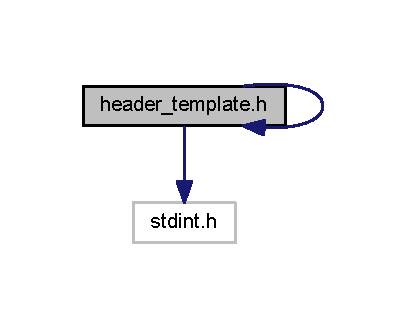
\includegraphics[width=195pt]{header__template_8h__incl}
\end{center}
\end{figure}
This graph shows which files directly or indirectly include this file\+:\nopagebreak
\begin{figure}[H]
\begin{center}
\leavevmode
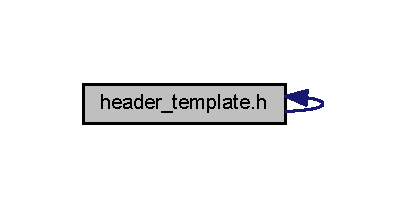
\includegraphics[width=195pt]{header__template_8h__dep__incl}
\end{center}
\end{figure}
\subsection*{Classes}
\begin{DoxyCompactItemize}
\item 
struct \hyperlink{struct_s_t_r_u___d_e_m_o}{S\+T\+R\+U\+\_\+\+D\+E\+MO}
\end{DoxyCompactItemize}
\subsection*{Macros}
\begin{DoxyCompactItemize}
\item 
\#define \hyperlink{header__template_8h_aacc3ee1a7f283f8ef65cea31f4436a95}{M\+AX}(x,  y)~(((x)$>$(y))?(x)\+:(y))
\item 
\#define \hyperlink{header__template_8h_a996f7be338ccb40d1a2a5abc1ad61759}{A\+BS}(x)~(((x) $>$ 0)?(x)\+:(-\/(x)))
\end{DoxyCompactItemize}
\subsection*{Enumerations}
\begin{DoxyCompactItemize}
\item 
enum \hyperlink{header__template_8h_ac927bbf88bd29dd0a1c7715df9fb443c}{E\+\_\+\+D\+E\+MO} \{ \hyperlink{header__template_8h_ac927bbf88bd29dd0a1c7715df9fb443ca87ef681eef180be8ed49aea2a997406b}{D\+E\+M\+O\+\_\+\+V\+A\+L\+UE} = 0, 
\hyperlink{header__template_8h_ac927bbf88bd29dd0a1c7715df9fb443ca0d3241fdf12699b594076d73f443f9ba}{D\+E\+M\+O\+\_\+\+V\+A\+L\+U\+E2} = 1
 \}
\end{DoxyCompactItemize}
\subsection*{Functions}
\begin{DoxyCompactItemize}
\item 
void \hyperlink{header__template_8h_ab518b0cc10ff8b098e2a2f145c8bacf7}{v\+\_\+function\+\_\+demo} (uint8\+\_\+t u8\+\_\+var1, uint32\+\_\+t u32\+\_\+var2)
\begin{DoxyCompactList}\small\item\em Description of function. \end{DoxyCompactList}\end{DoxyCompactItemize}


\subsection{Macro Definition Documentation}
\mbox{\Hypertarget{header__template_8h_a996f7be338ccb40d1a2a5abc1ad61759}\label{header__template_8h_a996f7be338ccb40d1a2a5abc1ad61759}} 
\index{header\+\_\+template.\+h@{header\+\_\+template.\+h}!A\+BS@{A\+BS}}
\index{A\+BS@{A\+BS}!header\+\_\+template.\+h@{header\+\_\+template.\+h}}
\subsubsection{\texorpdfstring{A\+BS}{ABS}}
{\footnotesize\ttfamily \#define A\+BS(\begin{DoxyParamCaption}\item[{}]{x }\end{DoxyParamCaption})~(((x) $>$ 0)?(x)\+:(-\/(x)))}

Computes absolute value of {\itshape x} \mbox{\Hypertarget{header__template_8h_aacc3ee1a7f283f8ef65cea31f4436a95}\label{header__template_8h_aacc3ee1a7f283f8ef65cea31f4436a95}} 
\index{header\+\_\+template.\+h@{header\+\_\+template.\+h}!M\+AX@{M\+AX}}
\index{M\+AX@{M\+AX}!header\+\_\+template.\+h@{header\+\_\+template.\+h}}
\subsubsection{\texorpdfstring{M\+AX}{MAX}}
{\footnotesize\ttfamily \#define M\+AX(\begin{DoxyParamCaption}\item[{}]{x,  }\item[{}]{y }\end{DoxyParamCaption})~(((x)$>$(y))?(x)\+:(y))}


\begin{DoxyCodeInclude}
\end{DoxyCodeInclude}
 more include here

Computes maximum of {\itshape x} and {\itshape y} 

\subsection{Enumeration Type Documentation}
\mbox{\Hypertarget{header__template_8h_ac927bbf88bd29dd0a1c7715df9fb443c}\label{header__template_8h_ac927bbf88bd29dd0a1c7715df9fb443c}} 
\index{header\+\_\+template.\+h@{header\+\_\+template.\+h}!E\+\_\+\+D\+E\+MO@{E\+\_\+\+D\+E\+MO}}
\index{E\+\_\+\+D\+E\+MO@{E\+\_\+\+D\+E\+MO}!header\+\_\+template.\+h@{header\+\_\+template.\+h}}
\subsubsection{\texorpdfstring{E\+\_\+\+D\+E\+MO}{E\_DEMO}}
{\footnotesize\ttfamily enum \hyperlink{header__template_8h_ac927bbf88bd29dd0a1c7715df9fb443c}{E\+\_\+\+D\+E\+MO}}

A description of the struct. \begin{DoxyEnumFields}{Enumerator}
\raisebox{\heightof{T}}[0pt][0pt]{\index{D\+E\+M\+O\+\_\+\+V\+A\+L\+UE@{D\+E\+M\+O\+\_\+\+V\+A\+L\+UE}!header\+\_\+template.\+h@{header\+\_\+template.\+h}}\index{header\+\_\+template.\+h@{header\+\_\+template.\+h}!D\+E\+M\+O\+\_\+\+V\+A\+L\+UE@{D\+E\+M\+O\+\_\+\+V\+A\+L\+UE}}}\mbox{\Hypertarget{header__template_8h_ac927bbf88bd29dd0a1c7715df9fb443ca87ef681eef180be8ed49aea2a997406b}\label{header__template_8h_ac927bbf88bd29dd0a1c7715df9fb443ca87ef681eef180be8ed49aea2a997406b}} 
D\+E\+M\+O\+\_\+\+V\+A\+L\+UE&Some documentation for first. \\
\hline

\raisebox{\heightof{T}}[0pt][0pt]{\index{D\+E\+M\+O\+\_\+\+V\+A\+L\+U\+E2@{D\+E\+M\+O\+\_\+\+V\+A\+L\+U\+E2}!header\+\_\+template.\+h@{header\+\_\+template.\+h}}\index{header\+\_\+template.\+h@{header\+\_\+template.\+h}!D\+E\+M\+O\+\_\+\+V\+A\+L\+U\+E2@{D\+E\+M\+O\+\_\+\+V\+A\+L\+U\+E2}}}\mbox{\Hypertarget{header__template_8h_ac927bbf88bd29dd0a1c7715df9fb443ca0d3241fdf12699b594076d73f443f9ba}\label{header__template_8h_ac927bbf88bd29dd0a1c7715df9fb443ca0d3241fdf12699b594076d73f443f9ba}} 
D\+E\+M\+O\+\_\+\+V\+A\+L\+U\+E2&Some documentation for sencond. \\
\hline

\end{DoxyEnumFields}


\subsection{Function Documentation}
\mbox{\Hypertarget{header__template_8h_ab518b0cc10ff8b098e2a2f145c8bacf7}\label{header__template_8h_ab518b0cc10ff8b098e2a2f145c8bacf7}} 
\index{header\+\_\+template.\+h@{header\+\_\+template.\+h}!v\+\_\+function\+\_\+demo@{v\+\_\+function\+\_\+demo}}
\index{v\+\_\+function\+\_\+demo@{v\+\_\+function\+\_\+demo}!header\+\_\+template.\+h@{header\+\_\+template.\+h}}
\subsubsection{\texorpdfstring{v\+\_\+function\+\_\+demo()}{v\_function\_demo()}}
{\footnotesize\ttfamily void v\+\_\+function\+\_\+demo (\begin{DoxyParamCaption}\item[{uint8\+\_\+t}]{u8\+\_\+var1,  }\item[{uint32\+\_\+t}]{u32\+\_\+var2 }\end{DoxyParamCaption})}



Description of function. 

Extern functions

Global functions


\begin{DoxyParams}[1]{Parameters}
\mbox{\tt in}  & {\em u8\+\_\+var1} & description for u8\+\_\+var1 \\
\hline
\mbox{\tt in}  & {\em u32\+\_\+var2} & description for u32\+\_\+var2 \\
\hline
\end{DoxyParams}
\begin{DoxyReturn}{Returns}
None 
\end{DoxyReturn}

%--- End generated contents ---

% Index
\backmatter
\newpage
\phantomsection
\clearemptydoublepage
\addcontentsline{toc}{chapter}{Index}
\printindex

\end{document}
